\documentclass[tikz,border=5pt]{standalone}
\usepackage{amsmath,amssymb}
\begin{document}
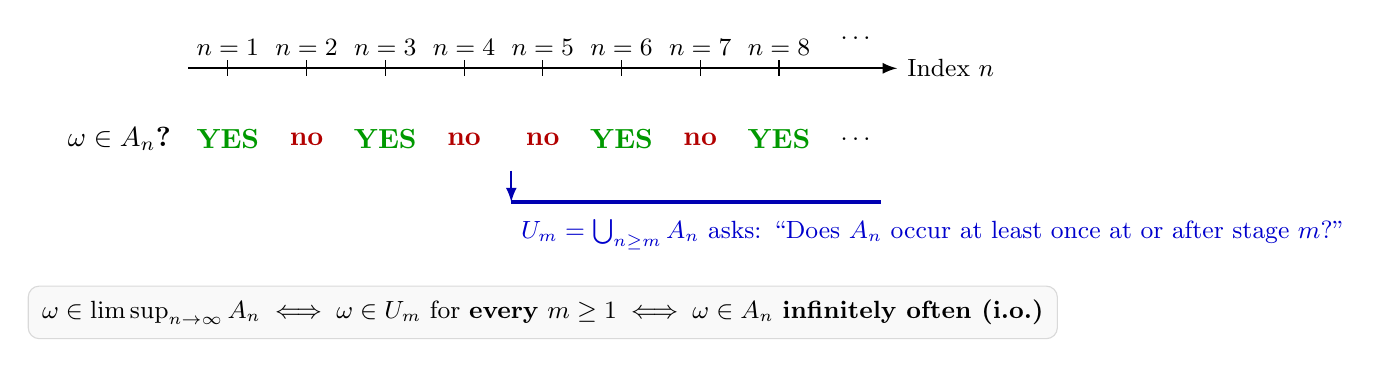
\begin{tikzpicture}[>=latex, font=\small]
  % Index axis
  \draw[->, thick] (0.5, 1.5) -- (9.5, 1.5) node[right] {Index $n$};
  
  \foreach \n in {1, 2, 3, 4, 5, 6, 7, 8} {
    \draw (\n, 1.6) -- (\n, 1.4) node[above=4pt] {$n=\n$};
  }
  \node[above=4pt] at (9, 1.6) {$\dots$};

  % Realization of omega
  \node[left, font=\bfseries] at (0.4, 0.6) {$\omega \in A_n$?};
  \node[font=\bfseries, color=green!60!black] at (1, 0.6) {YES};
  \node[font=\bfseries, color=red!70!black] at (2, 0.6) {no};
  \node[font=\bfseries, color=green!60!black] at (3, 0.6) {YES};
  \node[font=\bfseries, color=red!70!black] at (4, 0.6) {no};
  \node[font=\bfseries, color=red!70!black] at (5, 0.6) {no};
  \node[font=\bfseries, color=green!60!black] at (6, 0.6) {YES};
  \node[font=\bfseries, color=red!70!black] at (7, 0.6) {no};
  \node[font=\bfseries, color=green!60!black] at (8, 0.6) {YES};
  \node at (9, 0.6) {$\dots$};

  % Tail union U_m
  \draw[line width=1.5pt, blue!70!black] (4.6, -0.2) -- (9.3, -0.2);
  \draw[->, thick, blue!70!black] (4.6, 0.2) -- (4.6, -0.2);
  \node[anchor=north west, blue!80!black] at (4.6, -0.3)
    {$U_m = \bigcup_{n \ge m} A_n$ asks: ``Does $A_n$ occur at least once at or after stage $m$?''};

  \node[align=center, fill=gray!5, draw=gray!30, rounded corners, inner sep=5pt] at (5.0, -1.6)
    {$\omega \in \limsup_{n\to\infty} A_n \iff \omega \in U_m \text{ for \textbf{every} } m \ge 1 \iff \omega \in A_n \text{ \textbf{infinitely often (i.o.)}}$};
\end{tikzpicture}
\end{document}
